
% ##########################################################################################################
\documentclass[a4paper,12pt]{article}
% \usepackage{lipsum}
% \usepackage[columnwise]{lineno}
\usepackage{cxltx}
\usepackage[
left=30mm,
right=25mm,
top=15mm]{geometry}
% \usepackage[headheight=10mm]{geometry}
\usepackage{leading}
\usepackage{parskip}
\usepackage{xeCJK}
\usepackage{lscape} % needed for show-labels
% ..........................................................................................................
% a trick from http://tex.stackexchange.com/questions/16084/high-and-low-cjk-codepoints-in-a-single-xelatex-document
% to automatically select font based on glyph codepoint; note that in order for `zhspacing` to load at all,
% you must install both the SimSun and the SimHei font, even if those fonts are not listed in your font
% choices.
%
%   http://www.fontpalace.com/font-download/SimHei/
%   http://www.fontpalace.com/font-download/SimSun/
\usepackage{zhspacing}
\zhspacing
\newfontfamily\zhfont{Sun-ExtA}
\newfontfamily\verbatimfont[Scale=0.8]{Flow DejaVu Sans Mono}
\newfontfamily\zhcjkextbfont{sunflower-u-cjk-xb}
% \setCJKmainfont{Sun-ExtA}
% \newCJKfontfamily\cjkxbIdeographFont[Scale=1.05,AutoFakeBold=1]{sunflower-u-cjk-xb}
% ..........................................................................................................

\usepackage{fancyhdr}
% \usepackage{verbatim}
% \usepackage{fancyvrb}
% \renewcommand{\FancyVerbFormatLine}[1]{%
%   % \makebox[0cm][l]{$\Rightarrow$}#1%
%   % \fontsize{3mm}{3mm}%
%   \color{red}#1%
%   }
% \let\verbatim=\Verbatim
% \renewcommand\verbatim{\Verbatim}
\makeatletter
\renewcommand\verbatim@font{\color{DarkRed}\verbatimfont\leading{4mm}}%\fontsize{3mm}{3mm}}
\makeatletter
% necessary to capture Pandoc's LaTeX output which uses `\texttt` insted of `\verb`:
\renewcommand{\texttt}[1]{{\color{DarkRed}\verbatimfont\leading{4mm}#1}}

\usepackage{etoolbox}
\patchcmd{\quote}{\rightmargin}{\leftmargin 1em\rightmargin}{}{}
\usepackage{enumitem}
\setlist[itemize]{leftmargin=*,label=¶}

\setmainfont[
Mapping=tex-text,
BoldFont={Liberation Sans Bold},
BoldFeatures={Scale=0.8},
ItalicFont={EB Garamond 12 Italic},
% Ligatures={Historic,Rare,TeX},
Ligatures={TeX},
% Style={Swash,Historic},
CharacterVariant={11,5:0},% 11: make medieval digit `1` look different from small caps `i`
]{EB Garamond 12 Regular}



\newenvironment{jzrplain}{%
% ..........................................................................................................
% begin
  % thx to http://www.tug.org/TUGboat/tb28-1/tb88bazargan.pdf for the next two settings:
  \lineskiplimit=-10pt%
  \lineskip=0pt%
  \topskip=0pt%
  \setlength{\parskip}{4mm}%
  \setlength{\parindent}{0mm}%
  % \fontsize{\nominalfontsize}{\gridstrutlength}%
  \leading{5.5mm}
  % \makeatletter
  % \preto{\@verbatim}{\topsep=0pt \partopsep=0pt }
  % \makeatother
  }%
% end
  {\par}


\renewcommand{\CXLTXcliRoute}{cxltx/lib/cli}
\renewcommand{\CXLTXtempOutRoute}{/tmp/CXLTXtempout.tex}
\renewcommand{\CXLTXtempErrRoute}{/tmp/CXLTXtemperr.tex}
\renewcommand{\CXLTXhost}{localhost:8910}
% \newcommand{\nodeRun}[2]{\nodeRunScript{\CXLTXcliRoute}{#1}{#2}}

% \makeatletter
% \def\verbatim{\tiny\@verbatim \frenchspacing\@vobeyspaces \@xverbatim}
% \makeatother

\makeatletter
\renewcommand{\paragraph}{%
  \@startsection{paragraph}{4}%
  {\z@}{1ex \@plus 1ex \@minus .2ex}{-1em}%
  {\normalfont\normalsize\bfseries}%
}
\makeatother

% ##########################################################################################################
\begin{document}
\begin{jzrplain}






\begingroup
\pagestyle{empty}
\fontsize{10pt}{10pt}
\leading{3mm}

\centering
~\vspace{8\baselineskip}\\


\includegraphics[width=0.2\linewidth]{fleuron2.png}\\[\baselineskip]

{\relsize{8}%...............................................................................................

\CXLTXlong\\[0.5\baselineskip]
(\CXLTXebgaramondBig\kern0.1em)\\[1\baselineskip]

}{\relsize{5}%..............................................................................................


}{\relsize{5}%..............................................................................................

\textit{How to}\\[0.5\baselineskip]

}{\relsize{7}%..............................................................................................

Extend \LaTeX\\[0.5\baselineskip]

}{\relsize{5}%..............................................................................................

\textit{with}\\[0.5\baselineskip]

}{\relsize{6}%..............................................................................................

A Real\\
Programming Language\\[\baselineskip]
}%..........................................................................................................


\includegraphics[width=0.2\linewidth]{fleuron.png}\\
% \clearpage
% ~
% \clearpage

\endgroup

% \cleardoublepage\section{Introduction}\label{intro}


% {\relsize{1}\CXLTX}

% {\relsize{2}\CXLTX}

% {\relsize{3}\CXLTX}

% {\relsize{4}\CXLTX}

% {\relsize{2}\relsize{2}A}{\relsize{4}A}{\relsize{2}A}A

% \CXLTXlong, or \CXLTX\ for short...



\clearpage
\begingroup
\thispagestyle{empty}
\tableofcontents


{\em Conventions}: In this document, (most) command line / code stuff is {\color{DarkRed} printed in red},
while (most) remote command output is {\color{DarkGreen} printed in green}.




\endgroup

\clearpage
\href{https://github.com/loveencounterflow/cxltx/raw/master/cxltx-manual.pdf}{Click
here to read the full documentation}

\section{CoffeeXeLaTeX (CXLTX)}\label{coffeexelatex-cxltx}

\subsection{What is it? And Why?}\label{what-is-it-and-why}

Everyone who has worked with LaTeX knows how hard it can often be to get
seemingly simple things done in this Turing-complete markup language.
Let's face it, (La)TeX has many problems; the
\href{http://www.infoq.com/presentations/Simple-Made-Easy}{complectedness}
of its inner workings and the extremely uneven syntax of its commands
put a heavy burden on the average user.

The funny thing is that \textbf{while TeX is all about computational
text processing, doing math and string processing are often really hard
to get right} (not to mention that TeX has no notion of higher-order
data types, such as, say, lists).

Often one wishes one could just do a simple calculation or build a
typesetting object from available data \emph{outside} of all that makes
LaTeX so difficult to get right. Turns out you can already do that, and
you don't have to recompile TeX.

Most of the time, running TeX means to author a source file and have the
TeX executable convert that into a PDF. Of course, this implies reading
and writing of files and executing binaries. Interestingly for us, both
capabilities---file access and command execution---are made available to
user-facing side of TeX: writing to a file happens via the
\texttt{\textbackslash{}write} command, while input from a file is done
with \texttt{\textbackslash{}input}; command execution repurposes
\texttt{\textbackslash{}write}, which may be called with the special
stream number \texttt{18} (internally, TeX does almost everything with
registers that are sometimes given symbolic names; it also enumerates
`channels' for file operations, and reserves \#18 for writing to the
command line and executing stuff). This is how the
\texttt{\textbackslash{}exec} command is (in essence) defined in
\texttt{coffeexelatex.sty}:

\begin{verbatim}
\newcommand{\CXLTXtempOutRoute}{/tmp/coffeexelatex.tex}

\newcommand{\exec}[1]{%
  \immediate\write18{#1 > \CXLTXtempOutRoute}
  \input{\CXLTXtempOutRoute}
  }
\end{verbatim}

With some TeXs, its possible to avoid the temporary file by using
\texttt{\textbackslash{}@@input\textbar{}"dir"}, but XeTeX as provided
by TeXLive 2013 does not allow that. The temporary file does have an
advantage: in case TeX should halt execution because of an error, and
that error is due to a script with faulty output, you can conveniently
review the problematic source by opening the temporary file in your text
editor.

Besides \texttt{\textbackslash{}exec}, there is also
\texttt{\textbackslash{}execdebug} which captures the \texttt{stderr}
output of a command and renders it in red to the document in case any
output occurred there.

\subsection{TeX and NodeJS}\label{tex-and-nodejs}

\subsubsection{Method One: Spawning a \texttt{node}
process}\label{method-one-spawning-a-node-process}

The whole idea of CXLTX is to have some external program receive data
from inside a running TeX invocation, process that data, and pass the
result back to TeX.

The command given to \texttt{\textbackslash{}exec} could be anything;
for our purposes, we will concentrate on running
\href{http://nodejs.org}{NodeJS} programs. The simplest thing is to have
NodeJS evaluate a JavaScript expression and print out the result; the
\texttt{\textbackslash{}evaljs} command has been defined to do just
that:

\begin{verbatim}
\newcommand{\evaljs}[1]{\execdebug{node -p "#1"}}

% will insert `16 * 3 = 48` in TeX math mode (triggered by `$`):
$ 16 * 3 = \evaljs{16 * 3} $
\end{verbatim}

This technique is easily adapted to work with
\href{http://coffeescript.org}{CoffeeScript} (or any other language that
compiles to JS):

\begin{verbatim}
\newcommand{\evalcs}[1]{\execdebug{coffee -e "console.log #1"}}

% will insert `[1,4,9]`
\evalcs{ ( n * n for n in [ 1, 2, 3 ] ) }
\end{verbatim}

\paragraph{The Command Line Remote Command Interface
(CL/RCI)}\label{the-command-line-remote-command-interface-clrci}

Of course, evaluating one-liners will give you only so much power, so
why not execute more sizeable programs? That's what
\texttt{\textbackslash{}nodeRun} is for:

\begin{verbatim}
\usepackage[abspath]{currfile}
\newcommand{\CXLTXmainRoute}{../../lib/main}
\newcommand{\nodeRun}[2]{
  \exec{node "\CXLTXmainRoute" "\currfileabsdir" "\jobname" "#1" "#2"}}

% will insert `Hello, world!`
\nodeRun{helo}{world}
\end{verbatim}

\texttt{\textbackslash{}NodeRun} will run NodeJS with the following
arguments: \textbf{(1)} the route to our custom-made executable;
\textbf{(2)} the route to the parent directory where the currently
processed TeX source files are; \textbf{(3)} the current job name;
\textbf{(4)} a command name (first argument to
\texttt{\textbackslash{}nodeRun}); and, lastly, \textbf{(5)} optional
command arguments (second argument to \texttt{\textbackslash{}nodeRun}).

Observe that you may want to define your own routes in case the default
values do not match your needs; these can be easily done using
\texttt{\textbackslash{}renewcommand}:

\begin{verbatim}
\renewcommand{\CXLTXmainRoute}{../../lib/main}
\renewcommand{\CXLTXtempOutRoute}{/tmp/CXLTXtempout.tex}
\renewcommand{\CXLTXtempErrRoute}{/tmp/CXLTXtemperr.tex}
\end{verbatim}

\subsubsection{Method Two: Spawning
\texttt{curl}}\label{method-two-spawning-curl}

Spawning a subprocess to `outsource' a computing task is certainly not
the cheapest or fastest way to do stuff, as creating and taking down a
process is relatively costly.

More specifically, spawning \texttt{node} is both comparatively
expensive (in terms of memory) and slow. Also, the subprocess must run
on the same machine as the main process, and unless that subprocess
persisted some data (in a DB or in a file), the subprocess will run in a
stateless fashion.

Then again, since we're using NodeJS anyway: What's more obvious than to
make TeX communicate with a long-running HTTP server?

Now i've not heard of any way to make TeX issue an HTTP request on its
own behalf. But we already know we can issue arbitrary command lines, so
we certainly can spawn \texttt{curl localhost} to communicate with a
server. We still have to spawn a subprocess that way---but maybe
\texttt{curl} is both lighter and faster than \texttt{node}!? It
certainly is.

Here are some timings i obtained for running our simple echoing example,
once spawning \texttt{node}, and once spawning \texttt{curl}. The server
is a very simple \href{http://expressjs.com/}{Express} application;
except for the command line argument and HTTP parameter handling, the
same code is ultimately executed:

\begin{verbatim}
time node "cxltx/lib/main" "cxltx/doc/" "cxltx-manual" \
  "helo" "friends" \
  > "/tmp/CXLTXtempout.tex" 2> "/tmp/CXLTXtemperr.tex"

real  0m0.140s
real  0m0.082s
real  0m0.083s

time curl --silent --show-error \
  127.0.0.1:8910/foobar.tex/cxltx-manual/helo/friends \
  > "/tmp/CXLTXtempout.tex" 2> "/tmp/CXLTXtemperr.tex"

real  0m0.010s
real  0m0.011s
real  0m0.010s
\end{verbatim}

In so far these rather naïve benchmarks can be trusted, they would
indicate that fetching the same insignificant amount of data via
\texttt{curl} from a local server is around ten times as performant as
doing the same thing by spawning \texttt{node}. The reason for this is
partly attributable to the considerable size of the NodeJS binary
(respectively whatever actions are taken by NodeJS to ready itself).

Even doing \texttt{time node -p "1"} results in execution times of over
0.07s. Add to this the \texttt{curl} timings of around 0.01s, and you
roughly get the 0.08s needed to spawn \texttt{node} and get results---in
other words, \texttt{curl} itself seems to be quite fast.

The upshot of this is that using our first method we can call external
code at a frequency around 10 per second, but using the \texttt{curl}
method, we can get closer to almost 100 per second (depending on the
machine etc). The difference might matter if you plan to put out a
\emph{lot} of external calls, and since the typical way of getting TeX
source code right is running and re-running TeX a lot of times, doing it
faster may help greatly.

\paragraph{The HTTP Remote Command Interface
(H/RCI)}\label{the-http-remote-command-interface-hrci}

\begin{verbatim}
% This is the default setting for calling the CXLTX RCI:
\renewcommand{\node}{\nodeCurl}

\node{helo}{friends}
\end{verbatim}

\subsubsection{Security Considerations}\label{security-considerations}

Be aware that executing arbitrary code by way of mediation of a command
line like

\begin{verbatim}
xelatex --enable-write18 --shell-escape somefile.tex
\end{verbatim}

is inherently unsafe: a TeX file downloaded from somewhere could erase
your disk, access your email, or install a program on your computer.
This is what the \texttt{-{}-enable-write18} switch is for: it is by
default fully or partially disabled so an arbitrary TeX source gets
limited access to your computer.

If you're scared now, please hang on a second. I just want to tell you
\emph{you should be really, really scared}. Why? Because if you ever
downloaded some TeX source to compile it on your machine \textbf{even
without the \texttt{-{}-enable-write18} switch} you've already
\textbf{executed potentially harmful code}. Few people are aware of it,
but many TeX installations are quite `liberal' in respect to what TeX
sources---TeX programs, really---are allowed to do \emph{even in absence
of command line switches}, and, as a result, even people who are hosting
public TeX installations for a living are susceptible to malicious
code.*

\textbf{It is a misconception that TeX source is `safe' because `TeX is
text-based format'} (how stupid is that, anyway?); \textbf{the truth is
that by doing \texttt{latex xy.tex} you're executing code which may do
malicious things}. Period. That said, the papers linked below make it
quite clear that \texttt{-{}-enable-write18} just `opens the barn door',
as it were, but in fact, there are quite a few other and less well known
avenues for TeX-based malware to do things on your computer.

And please don't think you're safe just because you're not executing
anything but your own TeX source---that, in case you're using LaTeX, is
highly improbable: any given real-world LaTeX document will start with a
fair number of \texttt{\textbackslash{}usepackage\{\}} statements, and
each one of those refers to a source that is publicly accessible on the
internet and has been so for maybe five or ten or more years. Someone
might even have managed to place a mildly useful package on CTAN, one
that has some obfuscated parts designed to take over world leadership on
Friday, 13th---who knows?

\textbf{The fact that TeX is a programming language that works by
repeatedly re-writing itself does not exactly help in doing static code
analysis}; in fact, such code is called
`\href{http://en.wikipedia.org/wiki/Metamorphic_code}{metamorphic code}'
and is a well-known technique employed by computer viruses.

Tu further stress the importance of metamorphic coding principles, let's
consider the assessment of metamorphic algorithms in the context of
seriously commercial and other applications as made deceptively clear in
a recently published paper:

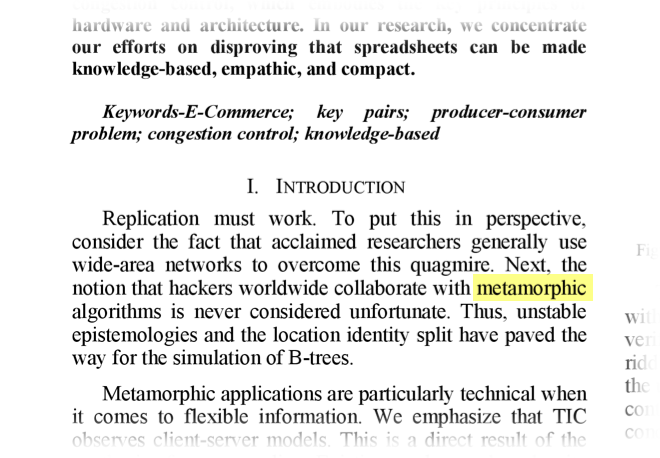
\includegraphics{cxltx/art/Screen Shot 2014-03-02 at 15.21.20.png} From
Zhang, Jing-Chun \& al, \emph{TIC: A methodology for the construction of
E-Commerce}; ©2013 IEEE

I do not write this section of the present README to scare you away,
just to inform whoever is concerned of a little known fact of life. The
gist of this is: don't have \texttt{-{}-enable-write18} turned on except
you know what you're doing, but be aware that running TeX has always
been unsafe anyway.

\begin{quote}
*) see e.g.
\texttt{http://cseweb.ucsd.edu/\textasciitilde{}hovav/dist/texhack.pdf}
\end{quote}

\subsection{Sample Command Lines}\label{sample-command-lines}

To make it easier for TeX to resolve
\texttt{\textbackslash{}usepackage\{cxltx\}}, put a symlink to your
CXLTX directory into a directory that is on LaTeX's search path. On OSX
with TeX Live, that can be achieved by doing

\begin{verbatim}
cd ~/Library/texmf/tex/latex
ln -s route/to/cxltx cxltx
\end{verbatim}

Here is what i do to build \texttt{cxltx/cxltx-manual.pdf}:

\textbf{(1)} use \href{http://http://johnmacfarlane.net/pandoc}{Pandoc}
to convert \texttt{README.md} to \texttt{README.tex}:

\begin{verbatim}
pandoc -o cxltx/doc/README.tex cxltx/README.md
\end{verbatim}

\textbf{(2)} copy the \texttt{aux} file from the previous TeX
compilation step to preserve its data for CXLTX to see:

\begin{verbatim}
cp cxltx/doc/cxltx-manual.aux cxltx/doc/cxltx-manual.auxcopy
\end{verbatim}

\textbf{(3)} compile \texttt{cxltx-manual.tex} to
\texttt{cxltx-manual.pdf} (\texttt{-{}-enable-write18}: allows to access
external programs form within TeX; \texttt{-{}-halt-on-error}: is a
convenience so i don't have to type \texttt{x} on each TeX error;
\texttt{-{}-recorder}: needed by the \texttt{currfile} package to get
absolute routes):

\begin{verbatim}
xelatex \
  --output-directory cxltx/doc \
  --halt-on-error \
  --enable-write18 \
  --recorder \
  cxltx/doc/cxltx-manual.tex
\end{verbatim}

\textbf{(4)} move the pdf file to its target location:

\begin{verbatim}
mv cxltx/doc/cxltx-manual.pdf cxltx
\end{verbatim}

\subsection{Useful Links}\label{useful-links}

http://www.ctan.org/tex-archive/macros/latex/contrib/perltex

http://ctan.space-pro.be/tex-archive/macros/latex/contrib/perltex/perltex.pdf

http://www.tug.org/TUGboat/tb28-3/tb90mertz.pdf

https://www.tug.org/TUGboat/tb25-2/tb81pakin.pdf

\subsection{Related Work}\label{related-work}

\begin{itemize}
\item
  \href{http://www.pytex.org/}{\textbf{PyTeX}} (also dubbed QATeX) is a
  laudable effort that has, sadly, been stalling for around 11 years as
  of this writing (January 2014), so it is likely pretty much outdated.
  PyTeX's approach is apparently the opposite of what we do in CXLTX:
  they run TeX in daemon mode from Python, where we have NodeJS start a
  server that listens to our independently running TeX.---Just for
  giggles, a quote from the above page: ``XML is hard work to key by
  hand. \emph{It lacks the mark-up minimization that SGML has}'' (my
  emphasis). Well, eleven years is a long time.
\item
  \href{https://github.com/gpoore/pythontex}{\textbf{PythonTeX}} is an
  interesting approach to bringing LaTeX and Python together.
  Unfortunately, the authors are preconcerned with showing off Pygment's
  syntax hiliting capabilities (which are \ldots{} not really that
  great) and how to print out integrals using SymPy; sadly, they fail to
  provide sample code of interest to a wider audience. Their copious
  128-page manual only dwells for one and a half page on the topic of
  `how do i use this stuff', and that only to show off more SymPy
  capabilities. None of their sample code \emph{needs} PythonTeX anyway,
  since none of it demonstrates how to interact with the document
  typesetting process; as such, all their formulas and plots may be
  produced offline, independently from LaTeX. Given that the
  installation instructions are too scary and longwinded for my taste,
  and that PythonTeX is not part of TeX Live, i've given up on the
  matter.
\end{itemize}

(the below taken from
http://get-software.net/macros/latex/contrib/pythontex):

\begin{itemize}
\item
  \href{http://www.ctan.org/tex-archive/macros/latex/contrib/sagetex}{\textbf{SageTeX}}
  allows code for the Sage mathematics software to be executed from
  within a \LaTeX~document.
\item
  Martin R. Ehmsen's
  \href{http://www.ctan.org/pkg/python}{\textbf{\texttt{python.sty}}}
  provides a very basic method of executing Python code from within a
  LaTeX document.
\item
  \href{http://elec.otago.ac.nz/w/index.php/SympyTeX}{\textbf{SympyTeX}}
  allows more sophisticated Python execution, and is largely based on a
  subset of SageTeX.
\item
  \href{http://www.luatex.org/}{\textbf{LuaTeX}} extends the pdfTeX
  engine to provide Lua as an embedded scripting language, and as a
  result yields tight, low-level Lua integration.
\end{itemize}

LuaTeX is one of the most interesting projects in this field as it
represents an attempt to provide a close coupling of a real programming
language with LaTeX. Unfortunately, that language is Lua, whose
designers believe that Unicode strings should be stored as UTF-8 bytes
(Go does the same, btw). Equally unfortunately, LuaTeX uses pdfTeX,
which can't compare to XeLaTeX when it comes to using custom TTF/OTF
fonts.


\clearpage
% \linenumbers


\clearpage%\mbox{}\clearpage

\section{Introduction}\label{intro}
% \lipsum[1]

(1) The original technique to execute an arbitrary command:
\begin{verbatim}
\immediate\write18{node
  "\CXLTXmainroute"
  "\currfilepath"
  "helo"
  "readers (one)"
  > /tmp/temp.dat}\input{/tmp/temp.dat}
\end{verbatim}

(2) With ugly details largely hidden, the \verb#\exec{}# command is still fully general:
\begin{verbatim}
\exec{node
  "\CXLTXmainroute"
  "\currfilepath"
  "helo"
  "readers (two)"}
\end{verbatim}

(3) \verb#\noderunscript{}# will execute NodeJS code that adheres to the call convention established by
\CXLTX:
\begin{verbatim}
\noderunscript
  {\CXLTXmainroute}
  {\currfilepath}
  {helo}
  {readers (three)}
\end{verbatim}

(4) Like the previous example, but with standard values assumed as shown above. This is the form that you
will want to use most of the time:
\begin{verbatim}
\noderun{helo}{readers (four)}
\end{verbatim}


{\textbf{Outputs:}}

\immediate\write18{node "\CXLTXmainroute" "\currfilepath" "helo" "readers (one)" > /tmp/temp.dat}\input{/tmp/temp.dat}

\exec{node "\CXLTXmainroute" "\currfilepath" "helo" "readers (two)"}

\noderunscript{\CXLTXmainroute}{\currfilepath}{helo}{readers (three)}

\noderun{helo}{readers (four)}

% ==========================================================================================================
\clearpage\section{Configuration}\label{config}

To use \CXLTX, put
\begin{verbatim}
\usepackage{coffeexelatex}
\end{verbatim}
into the header section of your \LaTeX\ file.

You may also want to include these lines in your \LaTeX\ document; these define, respectively, the route
to the \CXLTX\ executable (\verb#coffeexelatex/lib/main.js#) and the temporary file that is used to communicate
between \TeX\ and your scripts (relative routes are resolved with respect to the current working directory,
so if you set a relative route, you must always run \TeX\ from within the same directory):
\begin{verbatim}
\renewcommand{\CXLTXmainroute}{../../lib/main}
\renewcommand{\CXLTXtempoutroute}{/tmp/coffeexelatex.tex}
\end{verbatim}


% % ==========================================================================================================
% \clearpage\section{Geometry}\label{geo}

% % Write arbitrary text into the aux file:
% \auxc{this line goes to the aux file}

% % Write geometry data into the aux file:
% \auxgeo

% Use geometry data from aux file to render a table of layout dimensions into the document;
% note the we could have used the \verb#\auxgeo# command anywhere in the document and that
% this currently only works for documents with a single, constant layout.

% Also note we're using a dash instead of an underscore here—in \TeX, underscores are special, so
% we conveniently allow dashes to make things easier. The \CXLTX\ command \verb#show-geometry# does
% not take arguments, which is why the second pair of braces has been left empty:

% {\textbf{Command:}}
% \begin{verbatim}
% \noderun{show-geometry}{}
% \end{verbatim}

% {\textbf{Output:}}

% \noderun{show-geometry}{}

% ==========================================================================================================
\clearpage\section{Character Escaping}\label{esc}

The \CXLTX\ command \verb#show-special-chrs# demonstrates that it is easy to include \TeX\ special characters
in the return value. The simple rule is that whenever the output of a command is meant to be understood
literally, it should be \verb#@escape#d:

{\textbf{Command:}}

\begin{verbatim}
\noderun{show-special-chrs}{}
\end{verbatim}

{\textbf{Output:}}

\noderun{show-special-chrs}{}


% ==========================================================================================================
\clearpage\section{The \texttt{aux} Object}\label{aux}



% ----------------------------------------------------------------------------------------------------------
\subsection{Labels}\label{labels}

\CXLTX\ will try and collect all labels from the \verb#*.aux# file associated with the current job; from
inside your scripts 〓 〓 〓 〓 〓 〓 〓 〓 〓 〓 〓 〓 〓 〓 〓 〓 〓 〓 〓

{\textbf{Command:}}

\begin{verbatim}
\noderun{show-aux}{}
\end{verbatim}

{\textbf{Output:}}

{\fontsize{3mm}{3mm}\noderun{show-aux}{}}


% ----------------------------------------------------------------------------------------------------------
\subsection{Evaluating Expressions}\label{evalcs}

The commands \verb#\evalcs{}# and \verb#\evaljs{}# allow you to evaluate an arbitrary self-contained
expression, written either in CoffeeScript or in JavaScript:

{\textbf{Command:}}

\begin{verbatim}
$23 + 65 * 123 = \evalcs{23 + 65 * 123}$
\end{verbatim}

{\textbf{Output:}}

$23 + 65 * 123 = \evalcs{23 + 65 * 123}$


% ==========================================================================================================
\clearpage\section{Curl}\label{curl}
\begin{verbatim}
\curlRaw{127.0.0.1:8910/foobar.tex/helo/friends}
\end{verbatim}
\curlRaw{127.0.0.1:8910/foobar.tex/helo/friends}



% ----------------------------------------------------------------------------------------------------------
\subsection{Unicode}\label{unicode}

\begin{verbatim}
\curl{helo}{黎永強}
\end{verbatim}

\curl{helo}{黎永強}

\begin{verbatim}
\curl{helo}{äöüÄÖÜß}
\end{verbatim}

\curl{helo}{äöüÄÖÜß}

% ----------------------------------------------------------------------------------------------------------
\subsection{The URL environment}\label{urlenv}

Typing URLs in \LaTeX\ can be quite a chore, given the number of active and otherwise `special' characters
to take care of: not only does \TeX\ itself define some special characters, not only do the RFCs that govern
URL syntax consider 〓 〓 〓 〓 〓 〓 〓 〓 〓 〓 〓 〓 〓 〓 〓 〓 〓 〓 〓 special—when we communicate with our \CXLTX\ server,
we do so by executing a \verb#curl ...# command via the OS shell (normally \verb#sh#), which again has its own
rich set of specials. In order to alleviate the burden on the casual user, we define a new environment,
`URL`, that somewhat simplifies writing (parts of) URLs:
\begin{verbatim}
\begin{URL}
\curl{helo}{`\{ [ $ ~ % \# ^ | \} ] '?}
\end{URL}
\end{verbatim}
\begin{URL}
\curl{helo}{`\{ [ $ ~ % \# ^ | \} ] '?}
\end{URL}




% \begin{verbatim}
% \begin{URL}
% \curl{helo}{B \& C % Dollar: $ hash: \# caret: ^ wave:~ backtick: \` }
% \end{URL}
% \end{verbatim}
% \begin{URL}
% \curl{helo}{B \& C % Dollar: $ hash: \# caret: ^ wave:~ backtick: \` }
% \end{URL}

% \usepackage{textcomp} \textquotesingle \textasciigrave


% \CXLTXtemperrroute\ is \CXLTXiffileempty{\CXLTXtemperrroute}{indeed}{not} empty.
% \CXLTXtempoutroute\ is \CXLTXiffileempty{\CXLTXtempoutroute}{indeed}{not} empty.





% \begin{Verbatim}%
% [formatcom=\color{red}]
% First verbatim line.
% Second verbatim line.
% \end{Verbatim}

% % ----------------------------------------------------------------------------------------------------------
% \subsection{(testing)}

% \verb#\currfiledir#:  \currfiledir

% \verb#\currfilebase#: \currfilebase

% \verb#\currfileext#:  \currfileext

% \verb#\currfilename#: \currfilename

% \verb#\currfilepath#: \currfilepath

% \verb#\currfileabsdir#:   \currfileabsdir

% \verb#\currfileabspath#:  \currfileabspath

% % \begin{URL}
% \curlBETA{helo}{foo/bar}
% % \end{URL}

% \urlescapeALPHA{route/to/file}%
% \let\two=\urlescapecurrent%
% \two


% ##########################################################################################################
\end{jzrplain}
\end{document}
